\documentclass[../main.tex]{subfiles}
\begin{document}
\section{Metodología}
La metodología de la presente investigación se describe a continuación, detallando el diseño, los instrumentos, y las técnicas utilizadas para llevar a cabo el estudio.

\subsection{Diseño de la Investigación}

Esta investigación sigue un enfoque cuantitativo y experimental, complementado con elementos de aprendizaje por reproducción. Su propósito es analizar el funcionamiento de un modelo de red neuronal generativa adversaria profunda (GAN), replicar su implementación y estudiarlo para luego poder hacer algunas modificaciones. 

\subsection{Datos usados para el entrenamiento}\label{sec:dataset_explanation}

Los datos usados para el entrenamiento provienen de un dataset de \url{www.kaggle.com}, más concrétamente de un dataset llamado \textbf{Best Artworks of All Time} \cite{BestArtworksofAllTime2019}. Este dataset pesa 2.32 Gb y contiene imágenes de las pinturas de 49 artistas:

\begin{enumerate}
    \item Albrecht Durer (328 imágenes)
    \item Alfred Sisley (259 imágenes)
    \item Amedeo Modigliani (193 imágenes)
    \item Andrei Rublev (99 imágenes)
    \item Andy Warhol (181 imágenes)
    \item Camille Pissarro (91 imágenes)
    \item Caravaggio (55 imágenes)
    \item Claude Monet (73 imágenes)
    \item Diego Rivera (70 imágenes)
    \item Diego Velazquez (128 imágenes)
    \item Edgar Degas (702 imágenes)
    \item Edouard Manet (90 imágenes)
    \item Edvard Munch (67 imágenes)
    \item El Greco (87 imágenes)
    \item Eugene Delacroix (31 imágenes)
    \item Francisco Goya (291 imágenes)
    \item Frida Kahlo (120 imágenes)
    \item Georges Seurat (43 imágenes)
    \item Giotto di Bondone (119 imágenes)
    \item Gustav Klimt (117 imágenes)
    \item Gustave Courbet (59 imágenes)
    \item Henri Matisse (186 imágenes)
    \item Henri Rousseau (70 imágenes)
    \item Henri de Toulouse-Lautrec (81 imágenes)
    \item Hieronymus Bosch (137 imágenes)
    \item Jackson Pollock (24 imágenes)
    \item Jan van Eyck (81 imágenes)
    \item Joan Miro (102 imágenes)
    \item Kazimir Malevich (126 imágenes)
    \item Leonardo da Vinci (143 imágenes)
    \item Marc Chagall (239 imágenes)
    \item Michelangelo (49 imágenes)
    \item Mikhail Vrubel (171 imágenes)
    \item Pablo Picasso (439 imágenes)
    \item Paul Cezanne (47 imágenes)
    \item Paul Gauguin (311 imágenes)
    \item Paul Klee (188 imágenes)
    \item Peter Paul Rubens (141 imágenes)
    \item Pierre-Auguste Renoir (336 imágenes)
    \item Piet Mondrian (84 imágenes)
    \item Pieter Bruegel (134 imágenes)
    \item Raphael (109 imágenes)
    \item Rembrandt (262 imágenes)
    \item Rene Magritte (194 imágenes)
    \item Salvador Dali (139 imágenes)
    \item Sandro Botticelli (164 imágenes)
    \item Titian (255 imágenes)
    \item Vasiliy Kandinskiy (88 imágenes)
    \item Vincent van Gogh (877 imágenes)
    \item William Turner (66 imágenes)
    \item Marc Chagall (239 imágenes)
    \item Michelangelo (49 imágenes)
    \item Mikhail Vrubel (171 imágenes)
    \item Pablo Picasso (439 imágenes)
    \item Paul Cezanne (47 imágenes)
    \item Paul Gauguin (311 imágenes)
    \item Paul Klee (188 imágenes)
    \item Peter Paul Rubens (141 imágenes)
    \item Pierre-Auguste Renoir (336 imágenes)
    \item Piet Mondrian (84 imágenes)
    \item Pieter Bruegel (134 imágenes)
    \item Raphael (109 imágenes)
    \item Rembrandt (262 imágenes)
    \item Rene Magritte (194 imágenes)
    \item Salvador Dali (139 imágenes)
    \item Sandro Botticelli (164 imágenes)
    \item Titian (255 imágenes)
    \item Vasiliy Kandinskiy (88 imágenes)
    \item Vincent van Gogh (877 imágenes)
    \item William Turner (66 imágenes)
\end{enumerate}

Las distintas imágenes no tienen el mismo tamaño, por lo tanto hay que preprocesarlas antes de usarlas en el entrenamiento. 

\begin{figure}[htbp] % 'h' posiciona la figura cerca del texto
    \centering
    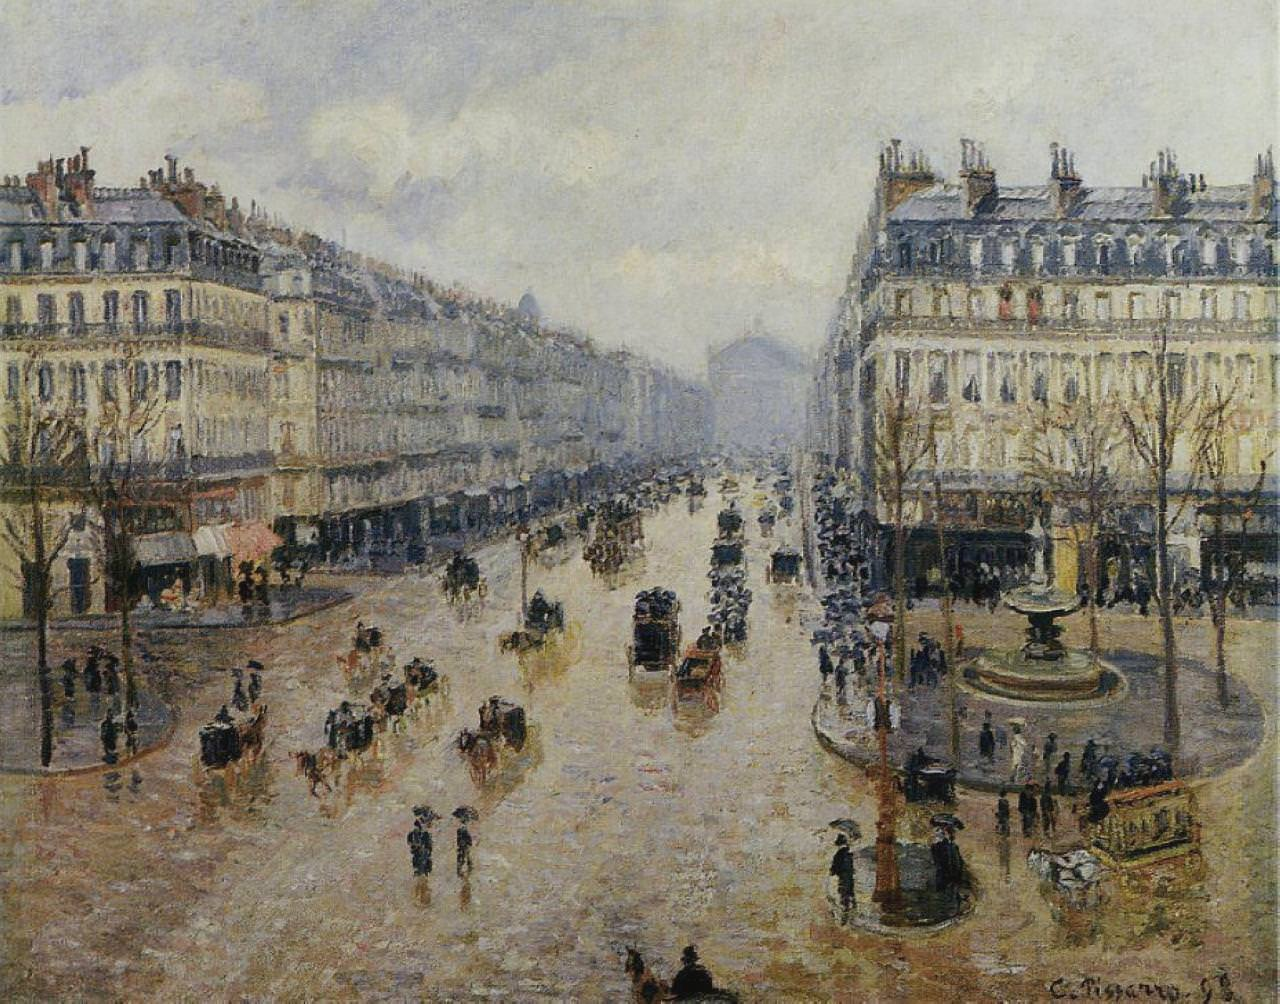
\includegraphics[width=\columnwidth]{Camille_Pissarro_12} % Ajuste al ancho de la columna
    \caption{Avenue de l'Opera Rain Effect de Camille Pissarro. 1898.}
    \label{fig:camille} % Etiqueta para referencia cruzada
\end{figure}

Una muestra del dataset la encontramos en la Figura~\ref{fig:camille}. Las distintas imágenes del dataset pertenecen a diferentes artistas de diferentes épocas. El más antiguo es Giotto di Bondone del año 1267–1337 y el más reciente es Andy Warhol  del año 1928–1987.

\subsection{Técnicas de Análisis de Datos}

Los datos serán analizados con diferentes herramientas, pero uso

\subsection{Instrumentos utilizados}

Los instrumentos utilizados en esta investigación incluyen:

\begin{itemize}
    \item \textbf{VSCode}: Como entorno de desarrollo para escribir y ejecutar el código.
    \item \textbf{Python}: Lenguaje de programación utilizado para la implementación del modelo GAN.
    \item \textbf{TensorFlow}: Biblioteca para la creación y entrenamiento de redes neuronales.
    \item \textbf{Numpy}: Biblioteca que usa los recursos de C para facilitar el cálculo con matrices.
    \item \textbf{Matplotlib}: Biblioteca para la graficación y mostrado de imágenes.
    \item \textbf{Pandas}: Biblioteca para el manejo
    eficiente de datos tabulares.
    \item \textbf{Pillow}: Biblioteca para la manipulación y mostrado de imágenes.
    \item \textbf{Keras}: API de redes neuronales escrita en Python, una interfaz de alto nivel.
    \item \textbf{Jupyter Nootebooks}: Aplicación que permite compilar y ejecutar código interactivo.
    \item \textbf{Anaconda}: Gestor de paquetes de Python orientado a la ciencia de datos.
\end{itemize}

La versión de \texttt{TensorFlow} es la 2.12.3 Por lo tanto, no se está usando la última versión disponible, si no la que es compatible con los demás paquetes según el administrador de paquetes de \texttt{Anaconda}.

\subsection{Procedimiento}
El procedimiento consistirá en tomar un modelo básico de GAN disponible en línea y adaptarlo a nuestras necesidades específicas. Primero, se realizará la preparación de los datos de entrenamiento utilizando un dataset de pinturas impresionistas. Luego, se entrenará el modelo, ajustando los parámetros según sea necesario para mejorar la calidad de las imágenes generadas. Finalmente, se evaluará la calidad de las imágenes generadas mediante métricas de similitud visual y análisis subjetivo.

\subsection{Ética de la Investigación}
Para esta investigación, se utilizarán pinturas de dominio público, específicamente del movimiento impresionista, lo que garantiza que no se infringirán derechos de autor. Además, se tomará en cuenta el uso ético de los datos, respetando las normativas vigentes sobre el uso de obras artísticas.

\subsection{Limitaciones}
Las principales limitaciones de esta investigación incluyen la falta de recursos computacionales avanzados, lo que puede limitar la capacidad de entrenamiento de redes neuronales complejas. Además, el conocimiento sobre redes neuronales es limitado, por lo que se intentará adaptar un código preexistente para ajustarlo a las necesidades del proyecto.

\end{document}
